\section{Séance 1 (MOSFET: Polarisation)}

\subsection{Exercice 1}
Première question qu'il faut se poser : s'agit-t-il d'un PMOS ou d'un NMOS?
La flèche se trouve au dessus, il s'agit donc d'un transistor de type PMOS.
Identifions ensuite les différents ports du transistor : la \textit{grille},
la \textit{source} et le \textit{drain}. La grille est facile à identifiée.
Pour un transitor de type PMOS, la source est toujours à une tension plus
élevée relativement au drain.

\begin{figure}[ht]
	\centering
	\begin{circuitikz} \draw
		(0,0) node[pmos](q1) {}
		(q1.G) node[anchor=east] {G $= V_{IN}$}
		(q1.S) node[anchor=east] {S}
		(q1.D) node[anchor=east] {D}
		(q1.D) node[anchor=west] {$V_{OUT}$}
	
		(q1.S) --++(0,0.5) node[vcc]{$V_{DD}$}
		(q1.D) to[R, l^=$R$, i=$I$] (0,-2.5) node[sground] {};
	\end{circuitikz}
\end{figure}

\paragraph{Caractéristique entée-sortie}

\begin{enumerate}
	\item Si $V_{IN} > \SI{4.2}{\volt}$, alors $V_{SG} < |V_{T0,p}| = \SI{0.8}{\volt}$
	et le transistor est coupé. Dans ce cas, $V_{OUT} = \SI{0}{\volt}$.
	\item Si $V_{IN} < \SI{4.2}{\volt}$, le transistor devient passant. Pour
	$V_{IN}$ encore proche de \SI{4.2}{\volt}, le courant $I$ sera encore
	petit. La tension $V_D = RI$ sera donc petite également, et donc la tension
	$V_{SD}$ sera grande. Le transistor sera donc en saturation.
	
	En saturation, et à condition de négliger l'effet \textsc{Early}, le courant
	traversant le transistor dépend de $V_{OV}^2$ et donc de $V_{SG}^2$. Si $V_{IN}$
	diminue, le courant dans le transistor, et donc $V_{OUT}$, augmente de manière
	quadratique.
	\item Avec l'augmentation de $V_{OUT} = V_D$, la tension $V_{SD}$ va diminuer
	progressivement. Le transistor va donc finir par passer en régime triode.
	On peut calculer pour quelle valeur de $V_{IN}$ le transistor passera de saturation
	à triode. Le point de changement est donné par
	\begin{align*}
		 V_{SD} & = V_{SG} - |V_{T0,p}| \\
		 V_{DD} - V_{OUT} & = V_{DD} - V_{IN} - 0.8 \\
		 V_{OUT} & = V_{IN} + 0.8 \\
		 RI & = V_{IN} + 0.8 \\
		 R\frac{k_p}{2}(V_{SG} - |V_{T0,p}|)^2 & = V_{IN} + 0.8 \\
		 R\frac{k_p}{2}(4.2 - V_{IN})^2 & = V_{IN} + 0.8.
	\end{align*}
	En connaissant $k_p$, on pourrait résoudre cette équation pour $V_{IN}$ et donc
	trouver pour quelle valeur de l'entrée le transistor passerait de saturation à triode.
\end{enumerate}

On peut se convaincre du résultat à l'aide d'une simulation \textsc{Spice}.

% TODO: en tikz ce sera plus beau !
\begin{figure}[ht]
	\centering
	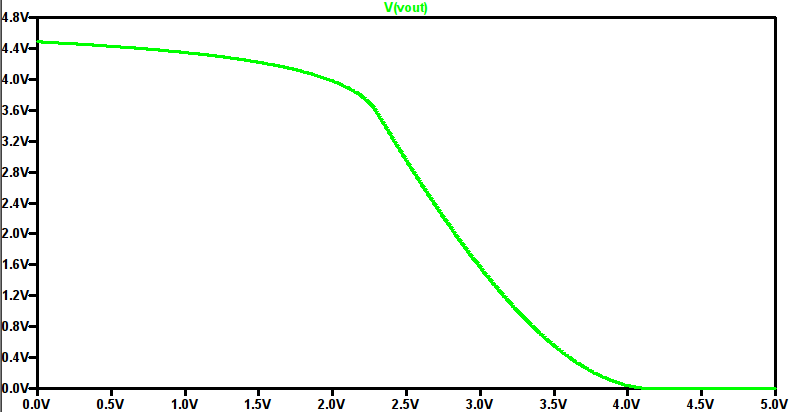
\includegraphics[scale=0.45]{exo1.png}
\end{figure}

\paragraph{Courbe $i_{SD}/v_{SD}$ et droite de charge}
Voir exemples dans les slides.

\section{Exercice 2}
\begin{enumerate}
	\item Pour calculer le courant $I$, étudions d'abord le régime de fonctionnement
	du transistor Q1. Il s'agit d'un transistor de type NMOS. Regardons ce qu'il se
	passe dans l'hypothèse où Q1 est bloqué (i.e. $V_{GS1}$ < $V_{T0,n} = \SI{1}{\volt}$).
	Dans ce cas, le courant $I$ est nul et la tension d'alimentation de \SI{5}{\volt} se
	retrouve entièrement sur le drain de $Q1$ : $V_{D1} = \SI{5}{\volt}$. Or, le drain
	et la grille de Q1 sont connectés et donc $V_{D1} = V_{G1} \Rightarrow V_{GS1}
	= \SI{5}{\volt}$, ce qui est en contradiction avec l'hyptohèse de départ. Q1 ne peut
	donc pas être bloqué.
	
	Il reste à déterminer si Q1 est en triode où en saturation. Pour cela, il faut
	comparer $V_{DS1}$ et $V_{OV1}$. Comme $V_{DS1} = V_{GS1}$ et $V_{OV1} = V_{GS1} -
	V_{T0,n}$, on a $V_{DS1} > V_{OV1}$ est Q1 est donc en saturation.
	\paragraph*{Remarque} Un transistor dont le drain est connecté à la grille est en
	fait toujours soit coupé, soit en saturation. On appelle cela un montage en diode.
	
	On trouve ensuite $I$ en résolvant le système	
	\[ I = \frac{\SI{5}{\volt}-V_{D1}}{\SI{270}{\kilo\ohm}} = \frac{k_n}{2}(V_{GS1} - 1)^2 =
	k_n(V_{D1} - 1)^2.\]	
	On obtient
	\[ V_{D1} = \SI{2.29}{\volt} \]
	et
	\[ I = \SI{10.04}{\micro\ampere}. \]
	
	\item Comme $V_{GS2}  = V_{GS1} = \SI{2.29}{\volt} > V_{T0,n}$, Q2 est passant. Pour aller
	plus loin, il faut faire une hypothèse et la vérifier a posteriori. On va ici supposer
	que Q2 est en saturation, c'est à dire que $V_{DS2} > V_{OV2} = V_{GS1} - V_{T0,n} =
	\SI{1.29}{\volt}$. Dans ce cas, en négligeant l'effet \textsc{Early}, le courant dans Q2
	ne dépend que de $V_{GS2}$. Comme de plus, Q1 et Q2 sont identiques et que $V_{GS1} = V_{GS2}$,
	on peut dire que le courant dans la branche de droite est identique au courant dans la branche
	de gauche.
	\paragraph{Remarque} Un tel montage est, pour cette raison, appelé "miroir de courant".
	
	\item Pour cela, il nous faut d'abord trouver le régime de fonctionnement de Q3. Comme
	$V_{SG3} = \SI{5}{\volt} > |V_{T0,p}| = \SI{1}{\volt}$, on peut déjà dire que Q3 est passant.
	
	A nouveau, il faut faire des hypothèses pour aller plus loin et les vérifier a posteriori.
	On suppose dans un premier temps que Q3 est en saturation, c'est à dire que $V_{SD3} >
	V_{SG3} - |V_{T0,p}| = \SI{4}{\volt}$. Dans ce cas,
	\[ \SI{10.04}{\micro\ampere} = \frac{k_p}{2}(V_{SG3} - 1)^2 \]
	et on trouve $V_{SG3} = \SI{3.24}{\volt}$. On a donc une contradiction puisqu'on sait que
	$V_{SG3} = \SI{5}{\volt}$ : Q3 ne peut donc être qu'en triode (i.e. $V_{SD3} < \SI{4}{\volt}$).
	Dans ce cas,
	\begin{align*}
		\SI{10.04}{\micro\ampere} 	& = k_p(V_{SG3} - |V_{T0,p}| - \frac{V_{SD3}}{2})V_{SD3} \\
									& = k_p(4 - \frac{(5 - V_{D3})}{2})(5-V_{D3}),
	\end{align*}
	et on a finalement
	\[ V_{D3} = V_{D2} = \SI{4.3}{\volt}.\]
	
	L'hypothèse de régime triode pour Q3 est donc bien vérifiée puisque $V_{SD3} = \SI{0.7}{\volt} < 
	\SI{4}{\volt}$. Il ne reste donc plus qu'à vérifier l'hypothèse prise pour Q2. Comme
	$V_{DS2} = \SI{4.3}{\volt} > V_{GS2} - V_{T0,n} = \SI{1.29}{\volt}$, Q2 est bel et bien
	en saturation.
	
	\item Voir questions précédentes.
\end{enumerate}

\section{Exercice 3}

\begin{enumerate}
	\item Le circuit a une relation linéaire entre le courant d'entrée et la tension de sortie:
	\[V_{out} = \alpha + \beta I_{in}.\]
	Cette relation sera démontrée dans les points suivants.

	On peut cependant analyser intuitivement le comportement du circuit: on suppose que les
	transistors sont en régime de saturation. Dès lors, en partant d'un état donné, si la tension
	$V_{out}$ augmente, $V_{gs1}$ augmente et $V_{gs2}$ diminue, et donc $I_{ds1}$ augmente tandis
	que $I_{ds2}$ diminue. Par Kirchoff, $I_{in}$ augmente.
	On peut appliquer le même raisonnement dans le cas où $V_{out}$ diminue. Par conséquent,
	$V_{out}$ suit les variations de $I_{in}$.
	
	\item Tout d'abord, on observe que le transistor Q1 est monté en diode. Il y a donc deux états
	possibles:
	\begin{itemize}
		\item bloqué si $V_{out} < V_{T0,n}$,
		\item en saturation si $V_{out} > V_{T0,n}$.
	\end{itemize}

	Pour Q2:
	\begin{itemize}
		\item bloqué si $V_{bias} - V_{out} < V_{T0,n}$,
		\item en saturation si $V_{bias} - V_{out} > V_{T0,n}$ et $V_{DD} - V_{out} > V_{bias} -
		V_{T0,n}$.
		\item en triode si $V_{bias} - V_{out} > V_{T0,n}$ et $V_{DD} - V_{out} < V_{bias} - V_{T0,n}$.
	\end{itemize}

	Dans le cas où $V_{DD} < V_{bias} - V_{T0,n}$, on peut passer de ces conditions sur la tension
	$V_{out}$ à des conditions sur le courant $I_{in}$ en utilisant les équations des transistors
	lorsqu'ils sont en saturation (plage de fonctionnement "normal" du circuit).

	\begin{align*}
    	I_1 &= \frac{k}{2}\left(V_{out} - V_{T0,n}\right)^2 \\
    	I_2 &= \frac{k}{2}\left(V_{bias} - V_{out} - V_{T0,n}\right)^2 \\
    	I_{1} &= I_{in} + I_{2}
	\end{align*}
    
	En résolvant ces équations, on trouve
	\[I_{in} = \frac{k}{2}\left(2 V_{T0,n} V_{bias} + (2 V_{bias} - 4 V_{T0,n}) V_{out} - V_{bias}
	^2\right)\]

	En prenant en compte la valeur de $V_{T0,n}$ et $V_{bias} = \SI{4}{V}$, on trouve
	\[I_{in} = k\left(\SI{2}{V} V_{out} - \SI{4}{V^2}\right)\]
	et donc
	\begin{itemize}
		\item si $I_{in} < -\SI{2}{V^2}k = -\SI{78}{\micro\ampere}$, Q1 est bloqué,
		\item si $I_{in} > \SI{2}{V^2}k = \SI{78}{\micro\ampere}$, Q2 est bloqué,
		\item sinon, les deux transistors sont en saturation.
	\end{itemize}

	\item Du point précédent, on trouve $-\SI{78}{\micro\ampere} < I_{in} < \SI{78}{\micro\ampere}$.

	\item Caractéristique:
	\begin{center}
		\includegraphics[width=0.6\textwidth,height=0.4\textwidth]{figures/ex3}
	\end{center}

	Equation de la caractéristique:
	\begin{itemize}
    	\item Si $I_{in} < \SI{-78}{\micro\ampere}$, Q1 est bloqué et
        \[I_{in} = - I_2 = -\frac{k}{2}\left(V_{bias} - V_{out} - V_{T0,n}\right)^2,\]
        donc \[V_{out} = V_{bias} - V_{T0,n} - \sqrt{\frac{2}{k}I_{in}}\]
    	\item Si $I_{in} > \SI{78}{\micro\ampere}$, Q2 est bloqué et
        \[I_{in} = I_1 = \frac{k}{2}\left(V_{out} - V_{T0,n}\right)^2,\]
        donc \[V_{out} = V_{T0,n} + \sqrt{\frac{2}{k}I_{in}}\]
	\end{itemize}
	
	\item On mesure la plage de fonctionnement linéaire par rapport à la sortie. La plage de
	fonctionnement linéaire s'étend entre $V_{T0,n}$ et $V_{bias} - V_{T0,n}$. On a donc une plage
	obtimale pour $V_{bias} = \SI{6}{V}$ (si $V_{bias} > \SI{6}{V}$, Q2 fonctionne en triode, et la
	relation entrée-sortie n'est plus linéaire).

	\item Si $k_1 \neq k_2$, on ne peut plus simplifier les termes en $V_{out}^2$ dans les équations
	(voir point 2), la relation entrée-sortie n'est donc plus linéaire.
\end{enumerate}

%Enoncé:
%k: 10^-5, pas 10^5
%point 2: en fonction de V_out et V_bias, puis I_in ? 
%k = k1 = k2
%point 2: extremement calculatoire en symbolique si V_bias quelconque => reformuler / fixer V_bias ?
%I_{in} < 0 : peu intéressant.

\end{document}